%\def\BRIEF{}  %indicates a short version

\documentclass[svgnames,12pt]{article}
\usepackage{graphicx}
\usepackage[dvipsn]{xcolor}
\usepackage{soul}
\usepackage{paralist}
\usepackage[T1]{fontenc}
\usepackage{textcomp}
\usepackage{bbding}
\usepackage{xstring}
\usepackage{stringstrings}
\usepackage{changepage}
\usepackage{titlesec}
\usepackage[hidelinks]{hyperref}
\definecolor{lstback}{RGB}{170, 220, 255}
%\usepackage{blindtext}
%\usepackage[scaled=.50]{helvet}
\usepackage[final]{listings}
\lstset{backgroundcolor=\color{lstback}}

\lstdefinestyle{CommandLineStyle}{
  basicstyle=\small\ttfamily,
  numbers=none,
  upquote=true % ensure that backtick displays correctly
}

\usepackage[a5paper, margin=0.4in, bottom=0.6in]{geometry}

\definecolor{syntaxcolor}{rgb}{0.6, 0, 0}
\definecolor{savedrescolor}{rgb}{0, 0.6, 0.4}
\definecolor{ecodecolor}{rgb}{1.0, 0.7, 0.7}
\sethlcolor{ecodecolor}

\newcommand{\minorheader}[1]{\vskip16pt{\color{ForestGreen}\textbf{#1}}}
\newcommand{\paramsheader}{\minorheader{Parameters}}
\newcommand{\optsheader}{\minorheader{Options}}
\newcommand{\savedres}{\minorheader{Saved results}}
\newcommand{\errheader}{\minorheader{Errors}}
\newcommand{\structheader}[1]{\minorheader{#1 frame data structure}}
\newcommand{\ecode}[1]{\texttt{\hl{ #1 }}}

\newcommand{\putimage}[1]{
  \ifdefined\BRIEF
  \else
  \begin{center}
      \includegraphics[width=\textwidth]{images/resized/#1}
  \end{center}
  \fi
}

\newcommand{\statacmd}[1]{
      \textbf{{\color{syntaxcolor}\texttt{#1}}}
}

\newcommand{\glossitem}[1]{
      \vskip8pt
      \textbf{{\color{syntaxcolor}\texttt{#1}}}
}

\newcommand{\option}[1]{{\color{syntaxcolor}\texttt{#1}}}
\newcommand{\savedresult}[1]{\vskip8pt{\color{savedrescolor}\texttt{#1}}}
\newcommand{\xmpl}[1]{\newline{\color{gray}\textit{\small#1\normalsize}}}

\let\oldsection\section
\renewcommand\section{\clearpage\oldsection}

\newcommand{\datafield}[1]{
    \vskip3pt
    \item[$\diamond$]
    {\color{blue}
      \textit{\getaword{#1}{1}}
      \textbf{\texttt{\getaword{#1}{2}}}
      \removeword[e]{#1}
      \removeword{\thestring}
    }
}


\titleformat{\section}
  {\normalfont\sffamily\Large\bfseries\color{cyan}}
  {\thesection}{1em}{}

\titleformat{\subsection}
  {\normalfont\sffamily\large\bfseries\color{cyan}}
  {\thesubsection}{1em}{}

\begin{document}
 \fontfamily{phv}\selectfont


\begin{titlepage}
   \vspace*{\stretch{2.0}}
   \begin{center}
      \Large\textbf{Survey Solutions API client for Stata}\\
      \vskip16pt
      \large\textit{S.Radyakin}\\
      \vskip16pt
      \large\textit{sradyakin@worldbank.org}\\
      \vskip186pt
      \today
   \end{center}
   \vspace*{\stretch{2.0}}
\end{titlepage}

\tableofcontents
    \section{Survey Solutions API Client for Stata}
\putimage{pexels-thisisengineering-3861943.jpg}

\vskip16pt
Survey Solutions API client for Stata is a software that facilitates the
control of a Survey Solutions data server from Stata scripts.

\vskip16pt
\subsection{Requirements}

\begin{itemize}
    \item \textbf{Stata 16.0} or newer.
    \item \textbf{Python 3.8} or newer (installed and accessible from Stata).
\end{itemize}

\vskip16pt
\subsection{Compatibility with The World Bank Survey Solutions:}
\begin{itemize}
  \item This software has been written with Survey Solutions v21.01.8 in mind,
        which is the current version at the time of this writing.
  \item Earlier versions may not implement all the functionality that is
        required for it, please update the Survey Solutions server.
  \item Future versions of Survey Solutions may change the behavior of the
        quieries or the formats of responses. If you encounter any
        incompatibility, please check the \href{https://docs.mysurvey.solutions/release_notes}{release notes} of Survey Solutions
        and see if an update is available for this API client.
\end{itemize}

\vskip16pt
\subsection{Installation}
\par
\vskip16pt
\textbf{Where to get:}\par
\begin{itemize}
  \item \textit{Stata:} \href{https://www.stata.com}{https://www.stata.com}
  \item \textit{Python:} \href{https://www.python.org/downloads/}{https://www.python.org/downloads/}
  \item \textit{This API client:} in Stata command prompt type \statacmd{ssc install susoapi}
  \item \textit{Survey Solutions server:} \href{https://mysurvey.solutions/download}{https://mysurvey.solutions/download}
\end{itemize}

\vskip16pt
\textbf{Checking Python from Stata.}\par
\vskip16pt
When you type the following command in Stata:\par
\vskip16pt
\begin{lstlisting}
python : import sys ; print(sys.version)
\end{lstlisting}
\vskip16pt
you should receive a response indicating Python version. For example: \par
\vskip16pt
\textit{3.8.1 (tags/v3.8.1:1b293b6, Dec 18 2019, 23:11:46) [MSC v.1916 64 bit (AMD64)]}.\par
\vskip16pt
If you are getting an error, then your Python installation is unusable from Stata. Refer to the Stata manual/support on how to install and configure Python for integration with Stata.

% todo: Add list of HTTP codes or a link to such a list.

\vskip16pt
\subsection{Dependencies}
\begin{center}
    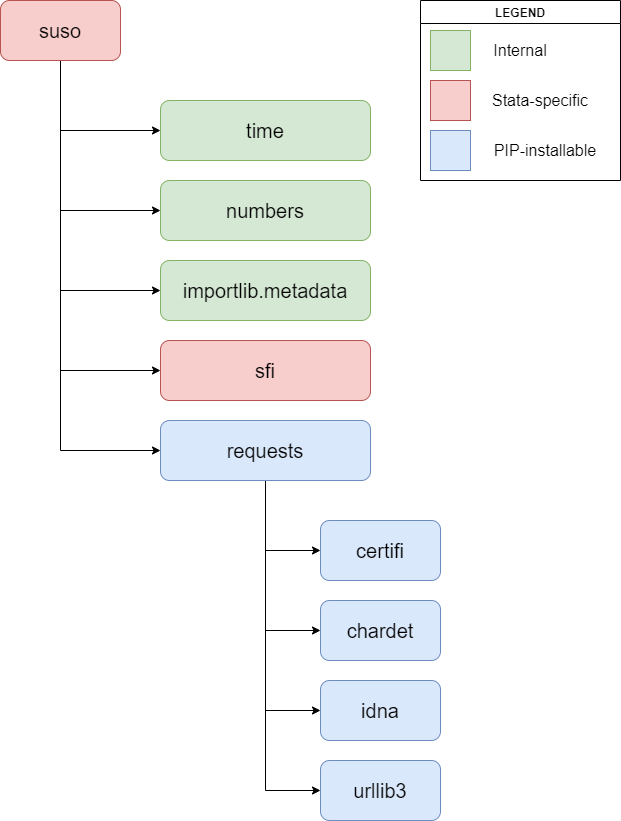
\includegraphics[width=70mm]{images/generated/susoapi-dependencies.png}
\end{center}


\vskip16pt
\subsection{Create a new API client}
\begin{lstlisting}
.new server username password
\end{lstlisting}

\paramsheader
\begin{itemize}
\item \option{server} - URL of the server, for example: \textquotedbl\textit{https://demo.mysurvey.solutions}\textquotedbl
\item \option{username} - name of the API user account, for example, \textquotedbl\textit{WeeklyAPI}\textquotedbl
\item \option{password} - API account password, for example, \textquotedbl\textit{VERY321secret}\textquotedbl
\end{itemize}

    \section{Questionnaires}
\putimage{pexels-alex-green-5699456.jpg}

\subsection{Get a list of questionnaires on the server}
\begin{lstlisting}[style=CommandLineStyle, showlines=true]

.qx_list, frame(string)

\end{lstlisting}

\optsheader
\begin{itemize}
  \item \option{frame} - (optional) frame name where to save the list. If not
  specified, the current frame is cleared and used to store the list.
\end{itemize}

\structheader{Questionnaires list}
\begin{compactitem}
  \datafield{str40 qx\_identity }
  \datafield{str32 qx\_id }
  \datafield{long  qx\_version }
  \datafield{strL  qx\_title }
  \datafield{str32 qx\_var }
  \datafield{strL  qx\_lastentry }
\end{compactitem}


\subsection{Get a list of interviews of a questionnaire on the server}

\begin{lstlisting}[style=CommandLineStyle, showlines=true]

.qx_interviews,
    qguid(string) qversion(integer)
    [frame(string)]

\end{lstlisting}

\optsheader
\begin{itemize}
  \item \option{qguid} - questionnaire GUID identifier.
  \item \option{qversion} - questionnaire version.
  \item \option{frame} - (optional) name of the frame to save the list of the
  interviews.
\end{itemize}

\structheader{Interviews list}
\begin{compactitem}
  \datafield{str36 interview\_\_id }
  \datafield{str36 qx\_guid }
  \datafield{long qx\_version }
  \datafield{long assignment\_id }
  \datafield{str36 responsible\_guid }
  \datafield{str36 responsible\_name }
  \datafield{long errors\_count }
  \datafield{str36 status }
  \datafield{strL lastentry }
  \datafield{byte received\_by\_device }
  \datafield{strL received\_by\_device\_at\_utc }
\end{compactitem}



\subsection{Get a questionnaire document in JSON format}

\begin{lstlisting}[style=CommandLineStyle, showlines=true]

.qx_document ,
    qguid(string) qversion(integer)
    saveto(string) [replace]

\end{lstlisting}

\optsheader
\begin{itemize}

    \item \option{qguid} - GUID of the questionnaire as a string, for example:
          \xmpl{"2d9d305f-fcc8-468c-9c7a-b3468d8204a7"}

    \item \option{qversion} - version of the questionnaire as imported
          to the HQ, numeric, for example:
          \xmpl{2}

    \item \option{saveto} - name of the file to be saved, for example:
          \xmpl{"C:/Temp/qx.json"}

    \item \option{replace} - (optional) allow overwriting the output file

\end{itemize}

\subsection{Set audio audit for the survey}
\begin{lstlisting}[style=CommandLineStyle, showlines=true]

.qx_setaudio qguid qversion value

\end{lstlisting}

\paramsheader
\begin{itemize}
    \item \option{qguid} - GUID of the questionnaire as a string, for example:
          \xmpl{"2d9d305f-fcc8-468c-9c7a-b3468d8204a7"}

    \item \option{qversion} - version of the questionnaire as imported
          to the HQ, numeric, for example:
          \xmpl{2}

    \item \option{value} - new mode of audio audit: \textit{1=ON} or
          \textit{0=OFF}, for example:
          \xmpl{1}

\end{itemize}

\subsection{Get status of audio audit for the survey}
\begin{lstlisting}[style=CommandLineStyle, showlines=true]

.qx_getaudio qguid qversion

\end{lstlisting}

\paramsheader
\begin{itemize}

    \item \option{qguid} - GUID of the questionnaire as a string, for example:
          \xmpl{"2d9d305f-fcc8-468c-9c7a-b3468d8204a7"}

    \item \option{qversion} - version of the questionnaire as imported
          to the HQ, numeric, for example:
          \xmpl{2}

\end{itemize}

\savedres
\begin{compactitem}

    \item \savedresult{r(record\_audio)} - numeric \textit{1=ON} or
    \textit{0=OFF}.

    \item \savedresult{r(status\_code)} - numeric status code for API query
    (successful completion is indicated by code 200).

\end{compactitem}

    \section{Assignments}
\putimage{pexels-pixabay-164686.jpg}





\subsection{Get a list of assignments on the server}
\begin{lstlisting}[style=CommandLineStyle]
.get_assignments, [qguid(string) qversion(integer)]
                  [responsible(string) supervisorid(string)]
                  [showarchive frame(string)]

\end{lstlisting}

\optsheader
\begin{itemize}
  \item \option{qguid} - questionnaire GUID identifier (optional, if not specified, no filtering by questionnaire or version is done).
  \item \option{qversion} - questionnaire version (optional, if not specified 1 is assumed, only effective when questionnaire GUID is specified).
  \item \option{responsible} - optional responsible name or GUID.
  \item \option{supervisorid} - optional supervisor GUID (not username).
  \item \option{showarchive} - regulates whether to search among active assignments (when this option is not specified, default) or archived assignments (when this option is specified).
  \item \option{frame} - (optional) name of the frame to save the list of the interviews.
\end{itemize}

\structheader{Assignments list}
\begin{compactitem}
  \datafield{long id } - for example: \textit{1064};
  \datafield{str36 responsible\_id } - identifier (GUID) of a person designated responsible
  for the assignment, for example: \textit{"1e7ef1e1-2123-4b5f-8a34-72ad1c494d1b"};
  \datafield{strL responsible\_name } - account name of a person designated responsible
  for the assignment, for example: \textit{"Natalia"};
  \datafield{strL questionnaireid } - for example: \textit{"8f1286c40c90475a9100b618584410b6\$1"};
  \datafield{long interviews\_count } - number of interviews assignment calls for, for example: \textit{10};
  \datafield{long quantity } - for example \textit{1};
  \datafield{byte archived } - 1 if the assignment is archived, 0 if not archived (active), for example \textit{0};
  \datafield{strL created\_at\_utc } - timestamp for when the assignment was created, in UTC, for example: \textit{"2024-03-19T23:48:04.358641Z"};
  \datafield{strL updated\_at\_utc } - timestamp for when the assignment was last updated, in UTC, for example: \textit{"2024-03-19T23:48:04.358641Z"};
  \datafield{strL email } - (for web assignments only) the email of the assignment recipient (respondent), for example: \textit{"somebody@somewhere.org"};
  \datafield{strL password } - (for web assignments only) the password to open the assignment (begin interview), for example: \textit{"PASS1234"};
  \datafield{byte webmode } - flag which indicates if the assignment is a web assignment (value is 1), or not (value is 0), for example: \textit{1};
  \datafield{strL received\_by\_tablet\_at\_utc } - timestamp for when the assignment was received by a mobile device, in UTC, for example: \textit{"2024-03-19T23:48:04.358641Z"};
  \datafield{byte is\_audio\_recording\_enabled } - 1 if audio audit is enabled for the assignment, 0 if not enabled, for example: \textit{0};
\end{compactitem}


\subsection{Get details of an assignment}

\begin{lstlisting}[style=CommandLineStyle]
.assignments_getdetails assignmentid
\end{lstlisting}

\paramsheader
\begin{itemize}
    \item \option{assignmentid} - numeric identifier of the assignment, for
    example: \textit{1007}.
\end{itemize}

\savedres
\begin{compactitem}
    \item r(CreatedAtUtc) - timestamp (date and time) of the creation of this
    assignment (in UTC), for example: \textit{"2021-05-17T14:41:46.824627Z"}.
    \item r(UpdatedAtUtc) - timestamp (date and time) of the last update (in
    UTC), for example: \textit{"2021-05-27T20:45:39.778723Z"}.
    \item r(QuestionnaireId)  - identity of the questionnaire on which this
    assignment is based. Identity is the questionnaire GUID and version
    separated with the \$ sign, for example: \newline
    \textit{"0434573c67b34d93b1f0799fb042f9e6\$1"}.
    \item r(ResponsibleName) - login name of the current responsible user,
    for example: \textit{"Natalia"}.
    \item r(ResponsibleId) - GUID of the current responsible user, for example:
    \textit{"71dc5a0f-6557-4945-9b86-0197699ee475"}.
\end{compactitem}

\vskip16pt
Additionally, for each identifying question, \#=1,2,...:
\begin{compactitem}
    \item r(id\_guid\#) - internally assigned GUID of the question,
    for example: \newline \textit{"c03979a9157304fcfa9bc1d3988433d7"}.
    \item r(id\_variable\#) - variable name for the question,
    for example: \textit{"province"}.
    \item r(id\_answer\#) - recorded answer to the identifying question,
    for example: \textit{"Northern province"}.
\end{compactitem}

\errheader
\begin{itemize}
    \item Error \ecode{5001} is returned if the \textit{assignmentid} is not specified.
    \item Error \ecode{5101} is returned if the \textit{assignmentid} is not a number (expected to be numberic).
    \item Error \ecode{5102} is returned if the \textit{assignmentid} is not 1 or more (expected to be 1 or a larger value).
    \item Error \ecode{5103} is returned if the \textit{assignmentid} is not an integer (expected to be an integer).
    \item Error \ecode{-10404} is returned if an assignment with \textit{assignmentid} is not found on the server.
\end{itemize}


\subsection{Assign an assignment to a new responsible}

\begin{lstlisting}[style=CommandLineStyle]
.assignments_assign assignmentid responsiblelogin
\end{lstlisting}

\paramsheader
\begin{itemize}
    \item \option{assignmentid} - numeric identifier of the assignment, for example: \textit{1007}.
    \item \option{responsiblelogin} - account name of the new responsible, for example: \textit{"Maryna"}.
\end{itemize}

\errheader
\begin{itemize}
    \item Error \ecode{5001} is returned if the \textit{assignmentid} is not specified.
    \item Error \ecode{5002} is returned if the \textit{responsiblelogin} is not specified.
    \item Error \ecode{5101} is returned if the \textit{assignmentid} is not a number (expected to be numberic).
    \item Error \ecode{5102} is returned if the \textit{assignmentid} is not 1 or more (expected to be 1 or a larger value).
    \item Error \ecode{5103} is returned if the \textit{assignmentid} is not an integer (expected to be an integer).
\end{itemize}



\subsection{Archive an assignment}

\begin{lstlisting}[style=CommandLineStyle]
.assignments_archive assignmentid
\end{lstlisting}

\paramsheader
\begin{itemize}
    \item \option{assignmentid} - numeric identifier of the assignment, for example: \textit{1007}.
\end{itemize}

\errheader
\begin{itemize}
    \item Error \ecode{5001} is returned if the \textit{assignmentid} is not specified.
    \item Error \ecode{5101} is returned if the \textit{assignmentid} is not a number (expected to be numberic).
    \item Error \ecode{5102} is returned if the \textit{assignmentid} is not 1 or more (expected to be 1 or a larger value).
    \item Error \ecode{5103} is returned if the \textit{assignmentid} is not an integer (expected to be an integer).
\end{itemize}



\subsection{Unarchive an assignment}

\begin{lstlisting}[style=CommandLineStyle]
.assignments_unarchive assignmentid
\end{lstlisting}

\paramsheader
\begin{itemize}
    \item \option{assignmentid} - numeric identifier of the assignment, for example: \textit{1007}.
\end{itemize}

\errheader
\begin{itemize}
    \item Error \ecode{5001} is returned if the \textit{assignmentid} is not specified.
    \item Error \ecode{5101} is returned if the \textit{assignmentid} is not a number (expected to be numberic).
    \item Error \ecode{5102} is returned if the \textit{assignmentid} is not 1 or more (expected to be 1 or a larger value).
    \item Error \ecode{5103} is returned if the \textit{assignmentid} is not an integer (expected to be an integer).
\end{itemize}


\subsection{Close an assignment}

\begin{lstlisting}[style=CommandLineStyle]
.assignments_close assignmentid
\end{lstlisting}

\paramsheader
\begin{itemize}
    \item \option{assignmentid} - numeric identifier of the assignment, for example: \textit{1007}.
\end{itemize}

\errheader
\begin{itemize}
    \item Error \ecode{5001} is returned if the \textit{assignmentid} is not specified.
    \item Error \ecode{5101} is returned if the \textit{assignmentid} is not a number (expected to be numberic).
    \item Error \ecode{5102} is returned if the \textit{assignmentid} is not 1 or more (expected to be 1 or a larger value).
    \item Error \ecode{5103} is returned if the \textit{assignmentid} is not an integer (expected to be an integer).
\end{itemize}



\subsection{Change quantity for an assignment}

\begin{lstlisting}[style=CommandLineStyle]
.assignments_changequantity assignmentid number
\end{lstlisting}

\paramsheader
\begin{itemize}
    \item \option{assignmentid} - numeric identifier of the assignment, for example: \textit{1007}.
    \item \option{number} - new quantity for the assignment, for example: \textit{10}.
\end{itemize}

\errheader
\begin{itemize}
    \item Error \ecode{5001} is returned if the \textit{assignmentid} is not specified.
    \item Error \ecode{5002} is returned if the \textit{number} is not specified.
    \item Error \ecode{5003} is returned if the \textit{number} is invalid (must be an integer, more than 0, 0, or -1).
    \item Error \ecode{5101} is returned if the \textit{assignmentid} is not a number (expected to be numberic).
    \item Error \ecode{5102} is returned if the \textit{assignmentid} is not 1 or more (expected to be 1 or a larger value).
    \item Error \ecode{5103} is returned if the \textit{assignmentid} is not an integer (expected to be an integer).
\end{itemize}


\subsection{Get quantity setting for an assignment}

\begin{lstlisting}[style=CommandLineStyle]
.assignments_getquantitysettings assignmentid
\end{lstlisting}

\paramsheader
\begin{itemize}
    \item \option{assignmentid} - numeric identifier of the assignment, for example: \textit{1007}.
    \item \option{number} - new quantity for the assignment, for example: \textit{10}.
\end{itemize}

\savedres
\begin{compactitem}
    \item r(can\_change\_quantity) - numeric 1=quantity can be changed or 0=quantity cannot be changed.
    \item r(status\_code)  - numeric status code for API query. Successful completion is indicated by code 200.
\end{compactitem}

\errheader
\begin{itemize}
    \item Error \ecode{5001} is returned if the \textit{assignmentid} is not specified.
    \item Error \ecode{5101} is returned if the \textit{assignmentid} is not a number (expected to be numberic).
    \item Error \ecode{5102} is returned if the \textit{assignmentid} is not 1 or more (expected to be 1 or a larger value).
    \item Error \ecode{5103} is returned if the \textit{assignmentid} is not an integer (expected to be an integer).
\end{itemize}


\subsection{Get audio audit status for an assignment}

\begin{lstlisting}[style=CommandLineStyle]
.assignments_getaudio assignmentid
\end{lstlisting}

\paramsheader
\begin{itemize}
    \item \option{assignmentid} - numeric identifier of the assignment, for example: \textit{1007}.
\end{itemize}

\savedres
\begin{compactitem}
    \item r(record\_audio) - numeric 1=ON or 0=OFF.
    \item r(status\_code)  - numeric status code for API query. Successful completion is indicated by code 200.
\end{compactitem}

\errheader
\begin{itemize}
    \item Error \ecode{5001} is returned if the \textit{assignmentid} is not specified.
    \item Error \ecode{5101} is returned if the \textit{assignmentid} is not a number (expected to be numberic).
    \item Error \ecode{5102} is returned if the \textit{assignmentid} is not 1 or more (expected to be 1 or a larger value).
    \item Error \ecode{5103} is returned if the \textit{assignmentid} is not an integer (expected to be an integer).
\end{itemize}

\subsection{Set audio audit status for an assignment}

\begin{lstlisting}[style=CommandLineStyle]
.assignments_setaudio assignmentid value
\end{lstlisting}

\paramsheader
\begin{itemize}
    \item \option{assignmentid} - numeric identifier of the assignment, for example: \textit{1007}.
    \item \option{value} - numeric value for the audio audit status of the assignment (0=OFF, any other value=ON), for example: \textit{1}.

\end{itemize}

\savedres
\begin{compactitem}
    \item r(record\_audio) - numeric 1=ON or 0=OFF.
    \item r(status\_code)  - numeric status code for API query. Successful completion is indicated by code 200.
\end{compactitem}

\errheader
\begin{itemize}
    \item Error \ecode{5001} is returned if the \textit{assignmentid} is not specified.
    \item Error \ecode{5002} is returned if the \textit{value} of audio audit is not specified.
    \item Error \ecode{5101} is returned if the \textit{assignmentid} is not a number (expected to be numberic).
    \item Error \ecode{5102} is returned if the \textit{assignmentid} is not 1 or more (expected to be 1 or a larger value).
    \item Error \ecode{5103} is returned if the \textit{assignmentid} is not an integer (expected to be an integer).
\end{itemize}

\subsection{Get assignment's history}

\begin{lstlisting}[style=CommandLineStyle]
.assignments_history assignmentid frame
\end{lstlisting}

\paramsheader
\begin{itemize}
    \item \option{assignmentid} - numeric identifier of the assignment, for example: \textit{1007}.
    \item \option{framename} - (optional) frame name where to save the assignment history, for example: \textit{"history"}. If not specified, the history is saved to the current frame.

\end{itemize}

\structheader{Assignment history}

\begin{compactitem}
    \datafield{str32 utc\_date } (for example, "\textit{2020-10-05T15:33:30.317233Z}")
    \datafield{str32 action } (for example, "\textit{Created}")
    \datafield{str32 actor\_name } (for example, "\textit{ValeriaHQ}")
    \datafield{strL additional\_data } (for example, "\textit{\{'Comment': None, 'Responsible': 'SergiyInt'\}}")
\end{compactitem}

\errheader
\begin{itemize}
    \item Error \ecode{5001} is returned if the \textit{assignmentid} is not specified.
    \item Error \ecode{5101} is returned if the \textit{assignmentid} is not a number (expected to be numberic).
    \item Error \ecode{5102} is returned if the \textit{assignmentid} is not 1 or more (expected to be 1 or a larger value).
    \item Error \ecode{5103} is returned if the \textit{assignmentid} is not an integer (expected to be an integer).
    \item Error \ecode{-10404} is returned if the assignment with \textit{assignmentid} is not found on the server.
\end{itemize}


\subsection{Create an assignment}

\begin{lstlisting}[style=CommandLineStyle]
.assignments_create , responsible() qxguid() [qxversion() quantity()]
             [email() password() webmode()]
             [audio() comment() protected() data()]
\end{lstlisting}

\optsheader
\begin{itemize}

\item \option{responsible} - account name of a person designated responsible
for the assignment, for example: \textit{SergiyInt}. NB: for web interviews the
responsible must be a user in the interviewer role.

\item \option{qxguid()} - GUID of the questionnaire.

\item \option{qxversion()} - (optional) numeric version of the questionnaire
      (as assigned when the questionnaire is imported to the HQ), for example:
      \textit{2}. When the option is not specified version 1 is implied.

\item \option{quantity()} - (optional) quantity of interviews requested in
      this assignment, for example: \textit{12}. When the option is not
      specified, quantity 1 is implied.

\item \option{email()} - (optional) respondent's email for sending the
      invitations and reminders for a web interview.

\item \option{password()} - (optional) password for accessing the web interview
      online.

\item \option{webmode()} - (optional) whether the assignment should be
      created in web mode. Specify 1 for web mode assignments, and 0 for regular
      assignments. If the option is not specified, regular assignments will be
      created.

\item \option{audio()} - (optional) whether audio audit should be collected for
      this assignment (1=on, 0=off). If the option is not specified, the audio
      audit will not be collected.

\item \option{comment()} - (optional) a comment to be recorded as an additional
      instruction regarding this assignment to the person who is designated
      responsible.

\item \option{protected()} - (optional) a space-delimited list of variables to
      be protected from modification by the interviewer (see the corresponding
      article in the documentation for Survey Solutions). For example,
      \textit{"memberscount plotslist"}. If the option is not specified, no
      variables are protected.

\item \option{data()} - (optional) output of the \textit{\textbf{.buildvars}}
      method or manually constructed preloading data in the same format, for
      example:
      \begin{lstlisting}[style=CommandLineStyle]
        `"{"Variable":"age", "Answer":41}"'
      \end{lstlisting}

\end{itemize}


NB: Remember to use Stata's compound double quotes to envelop the content in
the \textit{data()} option since it contains quotes of its own:

\begin{lstlisting}[style=CommandLineStyle]

local d = `"{"Variable":"region", "Answer":5}, "' + ///
  `"{"Variable":"address", "Answer":"1234 Test St., My City, USA"}"'

.s.assignments_create , ... data (`"`d'"')

\end{lstlisting}


\savedres
\begin{compactitem}
    \item r(status\_code) - numeric status code for the HTTP request corresponding to this query, for example \textit{201}; Successful completion is indicated by code 200 or 201.
    \item r(Id) - numeric assignment ID, for example: \textit{1226612};
    \item r(InterviewsCount) - number of interviews existing originating from this assignment, (expected always 0) for example: \textit{0};
    \item r(Archived) - numeric presentation of archival status (1=archived, 0=not archived), (expected always 0, not archived), for example: \textit{0};
    \item r(WebMode) - numeric presentation of the mode (1=Web mode, 0=Not web mode) for this assignment, for example: \textit{1};
    \item r(IsAudioRecordingEnabled) - flag whether audio recording is enabled for this assignment (1=ON or 0=OFF), for example: \textit(0);
    \item r(Email) - email of the web interview respondent, for example: \textit{"test@site.org"};
    \item r(CreatedAtUtc) - timestamp of the creation of the assignment (in UTC), for example: \textit{"2022-10-18T22:01:11.351222Z"};
    \item r(UpdatedAtUtc) - timestamp of the last update of the assignment (in UTC), for example: \textit{"2022-10-18T22:01:11.351222Z"}; (expected to be equal to timestamp of creation for newly created assignments);
    \item r(QuestionnaireId) - identity of the questionnaire (questionnaire ID and version), for example: \textit{"8352f83fe9eb4e48888142402a49ce3e\$1"};
    \item r(ResponsibleName) - login of the responsible, for example: \textit{"SergiyInt"};
    \item r(ResponsibleId) - GUID of the responsible, for example: \textit{"7607263d-ad66-4cc6-a175-42d3e6a57745"};
    \item r(WebInterviewLink) - web link to start an interview from this assignment, for example: \textit{"https://demo.mysurvey.solutions/census/WebInterview/V9FNU9PZ/Start"}.
\end{compactitem}

\errheader
\begin{itemize}
    \item Error \ecode{7001} is returned if the \textit{password} option is
    specified, but the assignment is created not in web mode (option webmode is
    0).

    \item Error \ecode{7002} is returned if the \textit{email} option is
    specified, but the assignment is created not in web mode (option webmode is
    0).

    \item Error \ecode{7003} is returned if the \textit{quantity} option is
    more than 1, but the assignment is created not in web mode (option webmode is
    0).

    \item Error \ecode{7004} is returned if the \textit{quantity} option is
    more than 10,000, which is a Survey Solutions limit for finite assignments.
\end{itemize}

    \section{Interviews}
\putimage{pexels-anna-shvets-5325100.jpg}

\subsection{Approve an interview by a supervisor}
\begin{lstlisting}[style=CommandLineStyle]
.interviews_approve guid [comment]
\end{lstlisting}
\paramsheader
\begin{itemize}
\item \option{guid} - GUID identifier of the interview to be approved.
\item \option{comment} - (optional) comment, if specified will be recorded as a comment to the transaction.
\end{itemize}

\subsection{Reject an interview by a supervisor}
\begin{lstlisting}[style=CommandLineStyle]
.interviews_reject guid [comment] [responsibleguid]
\end{lstlisting}
\paramsheader
\begin{itemize}
    \item \option{guid} - GUID identifier of the interview to be rejected.
    \item \option{comment} - (optional) comment, if specified will be recorded
          as a comment to the transaction.
    \item \option{responsibleguid} - (optional) GUID identifier of the new
          person responsible for the rejected interview.
\end{itemize}

\subsection{Unapprove an interview by a headquarters user}
\begin{lstlisting}[style=CommandLineStyle]
.interviews_hqunapprove guid [comment]
\end{lstlisting}
\paramsheader
\begin{itemize}
    \item \option{guid} - GUID identifier of the interview to be unapproved.
    \item \option{comment} - (optional) comment, if specified will be recorded
          as a comment to the transaction.
\end{itemize}

\subsection{Approve an interview by a headquarters user}
\begin{lstlisting}[style=CommandLineStyle]
.interviews_hqapprove guid [comment]
\end{lstlisting}
\paramsheader
\begin{itemize}
    \item \option{guid} - GUID identifier of the interview to be approved.
    \item \option{comment} - (optional) comment, if specified will be recorded
          as a comment to the transaction.
\end{itemize}

\subsection{Reject an interview by a headquarters user}
\begin{lstlisting}[style=CommandLineStyle]
.interviews_hqreject guid [comment] [responsibleguid]
\end{lstlisting}
\paramsheader
\begin{itemize}
    \item \option{guid} - GUID identifier of the interview to be rejected.
    \item \option{comment} - (optional) comment, if specified will be recorded
          as a comment to the transaction.
    \item \option{responsibleguid} - (optional) GUID identifier of the new
                person responsible for the rejected interview.
\end{itemize}

\subsection{Get a PDF document for the interview}
\begin{lstlisting}[style=CommandLineStyle]
.interviews_getpdf guid saveto
\end{lstlisting}
\paramsheader
\begin{itemize}
    \item \option{guid} - GUID identifier of the interview.
    \item \option{saveto} - name of the file where the PDF document
          for this interview must be saved.
\end{itemize}

\subsection{Get statistics for the interview}
\begin{lstlisting}[style=CommandLineStyle]
.interviews_getstats guid
\end{lstlisting}
\paramsheader
\begin{itemize}
    \item \option{guid} - GUID identifier of the interview.
\end{itemize}
\savedres
\begin{compactitem}
    \item r(InterviewId) - GUID of the interview, for example: \textit{"81784070-1e55-457c-b32e-b52d9672d9c4"};
    \item r(InterviewKey) - interview key, for example: \textit{"12-34-56-78"};
    \item r(Status) - status of the interview, for example: \textit{"Completed"};
    \item r(ResponsibleId) - GUID of the responsible person, for example: \textit{"39ad7fa7-4215-468b-9861-9a68b20662c2"}
    \item r(ResponsibleName) - login name of the current responsible, for example: \textit{"SergiyHQ"};
    \item r(InterviewDuration) - duration of the interview, for example: \textit{"00:14:48.3716360"}
    \item r(UpdatedAtUtc) - date and time of the last update to the interview data, for example: \textit{"2021-03-19T13:00:40.048662Z"};
    \item r(AssignmentId) - numeric assignment ID from which this interview has been started, for example: \textit{30711};
    \item r(NumberRejectionsByHq) - number of rejections by HQ user(s), for example: \textit{0}.
    \item r(NumberRejectionsBySupervisor) - number of rejections by supervisor user(s), for example: \textit{2}.
    \item r(NumberOfInterviewers) - number of interviewers that this interview was processed by, for example: \textit{1}.
    \item r(ForSupervisor) - number of supervisor questions, for example: \textit{3}.
    \item r(ForInterviewer) - number of questions for interviewer, for example: \textit{100}.
    \item r(WithComments) - number of questions with comments, for example: \textit{4}.
    \item r(Invalid) - number of questions with errors, for example: \textit{1}.
    \item r(Valid) - number of questions without errors, for example: \textit{99}.
    \item r(Flagged) - number of questions with flags, for example: \textit{0}.
    \item r(NotFlagged) - number of questions without flags, for example: \textit{100}.
    \item r(Answered) - number of questions which have been answered, for example: \textit{93}.
    \item r(NotAnswered) - number of questions which have not been answered, for example: \textit{7}.
\end{compactitem}

\subsection{Get history of the interview}
\begin{lstlisting}[style=CommandLineStyle]
.interviews_gethistory guid framename
\end{lstlisting}
\paramsheader
\begin{itemize}
    \item \option{guid} - GUID identifier of the interview.
    \item \option{framename} - (optional) name of the frame where the history
          of the interview must be saved. If not specified, the current frame
          is used.
\end{itemize}
\textbf{Interview history frame data structure}
\begin{compactitem}
    \datafield{string* timestamp } (for example, "\textit{2021-03-19T13:00:13.263127Z}")
    \datafield{string* offset } (for example, "\textit{-04:00:00}")
    \datafield{string* action } (for example, "\textit{Created}")
    \datafield{string* originator\_name } (for example, "\textit{MariaHQ}")
    \datafield{string* originator\_role } (for example, "\textit{Interviewer}")
    \datafield{string* parameters } (for example, "\textit{\{'question': 'OPZ401Q', 'answer': '750000', 'roster': '1,3'\}}")
\end{compactitem}
*NB: The exact storage types of the string variables depend on the content
     length and may vary.

\subsection{Get answers of the interview}
\begin{lstlisting}[style=CommandLineStyle]
.interviews_getanswers guid framename
\end{lstlisting}
\paramsheader
\begin{itemize}
    \item \option{guid} - GUID identifier of the interview.
    \item \option{framename} - (optional) name of the frame where the answers
          of the interview must be saved. If not specified, the current frame
          is used.
\end{itemize}
\textbf{Interview answers frame data structure}
\begin{compactitem}
    \datafield{string* variablename } (for example, "\textit{hhsize}")
    \datafield{str36 questionid } (for example, "\textit{50756294-eca7-4765-b94d-2f607dc049a0}")
    \datafield{string* rostervector } (for example, "\textit{[1, 3]}")
    \datafield{strL answer } (for example, "\textit{6}")
\end{compactitem}

*NB: The exact storage types of the string variables depend on the content
     length and may vary.

\subsection{Delete an interview}
\begin{lstlisting}[style=CommandLineStyle]
.interviews_delete guid
\end{lstlisting}
\paramsheader
\begin{itemize}
    \item \option{guid} - GUID identifier of the interview.
\end{itemize}
\errheader
\begin{itemize}
    \item Error \ecode{197} is returned if the \textit{guid} is not specified.
    \item Error \ecode{10101} is returned if the interview with ID \textit{guid} is not found.
    \item Error \ecode{10102} is returned if the interview with ID \textit{guid} may not be deleted.
\end{itemize}

\subsection{Assign an interview}
\begin{lstlisting}[style=CommandLineStyle]
.interviews_assign intguid responsibleguid
\end{lstlisting}
\paramsheader
\begin{itemize}
    \item \option{intguid} - GUID identifier of the interview.
    \item \option{responsibleguid} - GUID identifier of the new responsible.
\end{itemize}

\subsection{Assign supervisor/team to an interview}
\begin{lstlisting}[style=CommandLineStyle]
.interviews_supervisorassign intguid responsibleguid
\end{lstlisting}
\paramsheader
\begin{itemize}
    \item \option{intguid} - GUID identifier of the interview.
    \item \option{responsibleguid} - GUID identifier of the new responsible.
\end{itemize}


\subsection{Add a comment to a question in the interview by question GUID}
\begin{lstlisting}[style=CommandLineStyle]
.interviews_comment, interviewguid() questionguid()
                        comment() [rostervector()]
\end{lstlisting}
\optsheader
\begin{itemize}
    \item \option{interviewguid()} - GUID identifier of the interview.
    \item \option{questionguid()} - GUID identifier of the question where the
           comment must be added. NB: if GUID of the question is not known,
           see next section 4.14 for the equivalent method utilizing the
           variable name instead.
    \item \option{comment()} - text of the comment that must be added, for
           example: \textit{comment("Strange value")}
    \item \option{rostervector()} - rostervector address of the item if the
           question is part of the roster, for example: \textit{rostervector(5)}.
           NB: \textit{rostervector()} (if specified) is expected to be
           formatted according to the Survey Solutions rules: specifically
           as \#, or \#-\#, or \#-\#-\#, or \#-\#-\#-\#.
\end{itemize}

\subsection{Add a comment to a question in the interview by variable name}
\begin{lstlisting}[style=CommandLineStyle]
.interviews_varcomment, interviewguid() varname()
                        comment() [rostervector()]
\end{lstlisting}
\optsheader
\begin{itemize}
    \item \option{interviewguid()} - GUID identifier of the interview.
    \item \option{varname()} - variable name of the question where the
           comment must be added. NB: if varname of the question is not known,
           see previous section 4.13 for the equivalent method utilizing the
           question GUID instead.
    \item \option{comment()} - text of the comment that must be added,
           for example: \textit{comment("Strange value")}
    \item \option{rostervector()} - rostervector address of the item if the
           question is part of the roster, for example:
           \textit{rostervector(5)}. NB: \textit{rostervector()} (if specified)
           is expected to be formatted according to the Survey Solutions rules:
           specifically as \#, or \#-\#, or \#-\#-\#, or \#-\#-\#-\#.
\end{itemize}

    
\section{Data export}
\putimage{pexels-anete-lusina-4792750.jpg}
\subsection{Download data export file}
\begin{lstlisting}[style=CommandLineStyle, showlines=true]

.export2 ,
    qid() saveto() [replace]
    [translationid() includemeta]
    [status() exporttype()]
    [from() to()]

\end{lstlisting}

Exports data from Survey Solutions server based on the v2 data export (available
in Survey Solutions version 20.07 or newer).

\optsheader
\begin{itemize}
    \item \option{qid} - questionnaire identity, for example:
    \xmpl{"50756294-eca7-4765-b94d-2f607dc049a0\$13"}

    \item \option{saveto} - name of the file to save the exported date, for example:
    \xmpl{"C:/data/export.zip"}

    \item \option{replace} - (optional) if specified, allows to overwrite the
    file if it already exists.

    \item \option{translationid} - (optional) GUID of the translation of the
    questionnaire, for example:
    \xmpl{"2075f291-eca2-4965-b24d-7f607dc049e2"}

    \item \option{includemeta} - (optional) if specified this option requests
    meta-information to be included in the export file (specify
    \textit{"true"} to include, and \textit{"false"} to exclude the metadata).
    If not specified, the meta-information about the questionnaire
    (JSON-document, PDF-documents, etc) is excluded.

    \item \option{status} - (optional) filter by interview status. If specified,
    exported interviews data will be restricted to the data from interviews in
    that status, otherwise by default the data from all interviews is exported.

    \item \option{exporttype} - (optional) type of data file requested for
    export, can be one of the data types listed below. For example:
    \xmpl{Paradata} \newline
    If not specified, then \textit{"STATA"} is assumed.

    \item \option{from} - (optional), if specified, restricts the export to
    interviews modified since the specified date, for example:
    \xmpl{"2021-01-01T19:23:43.375Z"} \newline
    NB: if option \option{from()} is specified, then option \option{to()} must
    also be specified.

    \item \option{to} - (optional), if specified, restricts the export to
    interviews modified before the specified date, for example:
    \xmpl{"2021-01-01T19:23:43.375Z"} \newline
    NB: if option \option{to()} is specified, then option \option{from()} must
    also be specified.

\end{itemize}

\textbf{Data types for export files:}
\begin{compactitem}
    \item \statacmd{"Tabular"} - tab-delimited survey data (*.tab);
    \item \statacmd{"STATA"} - survey data in Stata format (*.dta);
    \item \statacmd{"SPSS"} - survey data in SPSS format (*.sav);
    \item \statacmd{"Binary"} - binary survey data (images, audio recordings);
    \item \statacmd{"DDI"} - DDI descriptor of the data;
    \item \statacmd{"Paradata"} - survey paradata.
\end{compactitem}

\par
\vskip24pt
\textbf{Statuses for the status filter:}
\begin{compactitem}
    \item \statacmd{"All"}
    \item \statacmd{"InterviewerAssigned"}
    \item \statacmd{"Completed"}
    \item \statacmd{"ApprovedBySupervisor"}
    \item \statacmd{"ApprovedByHeadquarters"}
\end{compactitem}

    \section{Maps}

\putimage{pexels-andrew-neel-2859169.jpg}

\subsection{Upload a map to the server.}
\begin{lstlisting}[style=CommandLineStyle]
.maps_uploadmaps , mapsfile(string) frame(string)
\end{lstlisting}

Call this API endpoint to upload a map to the server. The map must then be
assigned to one or more interviewers by calling the \textbf{.maps\_addusertomap}
endpoint. The zip archive containing the maps may include one or multiple maps,
including maps of different types (such as maps in .tpk, .mmpk, .tiff, etc formats).

NB: use the forward slash '\slash' rather than backward slash '\textbackslash' for
separating the folders in the path to file in the \textit{mapsfile} parameter.

\paramsheader
\begin{itemize}
  \item \option{mapsfile} - name of the zip archive containing one or multiple
        map files to be uploaded to the server, for example, \textquotedbl
        \textit{newmaps.zip}\textquotedbl, if the file is not in the current
        directory, include the full path to the file, for example, \textquotedbl
        \textit{C:/data/gis/maps/newmaps.zip}\textquotedbl;
  \item \option{frame} - name of a new frame that will be created to contain
        information about the individual map files that were uploaded, for
        example \textquotedbl \textit{loadedmaps}\textquotedbl.
\end{itemize}

\errheader
\begin{itemize}
    \item Error \ecode{5001} is returned if the server does not support
    maps uploading.
\end{itemize}

\savedres
\begin{compactitem}
    \item r(nMapsUploaded) - number of successfully uploaded maps.
\end{compactitem}



\subsection{Get list of maps and maps-to-user assignments}
\begin{lstlisting}[style=CommandLineStyle]
.maps_getmaps maps [users]
\end{lstlisting}

\paramsheader
\begin{itemize}
  \item \option{maps} - frame name for placing the list of maps currently on the server
  \item \option{users} - (optional) frame name for placing the list of users-to-maps assignments.
\end{itemize}

\structheader{Maps}
\begin{compactitem}
  \datafield{string* filename }
  \datafield{string* importdateutc }
  \datafield{long size }
  \datafield{long users }
  \datafield{long wkid }
  \datafield{double minscale }
  \datafield{double maxscale }
  \datafield{double xminval }
  \datafield{double xmaxval }
  \datafield{double yminval }
  \datafield{double ymaxval }
\end{compactitem}
*NB: The exact storage types of the string variables depend on the content
     length and may vary.

\structheader{User-maps}
\begin{compactitem}
  \datafield{string* filename }
  \datafield{string* username }
\end{compactitem}
*NB: The exact storage types of the string variables depend on the content
     length and may vary.


\subsection{Add an assignment of a map to a user.}
\begin{lstlisting}[style=CommandLineStyle]
.maps_addusertomap map user
\end{lstlisting}

\paramsheader
\begin{itemize}
  \item \option{map} - name of the map from the list of maps
        currently on the server, for example, \textquotedbl
        \textit{ukraine.tif}\textquotedbl
  \item \option{user} - interviewer account name, for example
        \textquotedbl SergiyInt\textquotedbl.
\end{itemize}


\subsection{Delete an assignment of a map from a user.}
\begin{lstlisting}[style=CommandLineStyle]
.maps_deleteuserfrommap map user
\end{lstlisting}

\paramsheader
\begin{itemize}
  \item \option{map} - name of the map from the list of maps currently on
        the server, for example, \textquotedbl \textit{ukraine.tif}\textquotedbl
  \item \option{user} - interviewer account name, for example \textquotedbl
        SergiyInt\textquotedbl.
\end{itemize}


\subsection{Delete a map from the server.}
\begin{lstlisting}[style=CommandLineStyle]
.maps_deletemap map
\end{lstlisting}

\paramsheader
\begin{itemize}
  \item \option{map} - name of the map from the list of maps currently on
  the server, for example, \textquotedbl \textit{ukraine.tif}\textquotedbl
\end{itemize}

    \input{s_notice.tex}
    \section{Users and user accounts}
\putimage{pexels-fauxels-3183150.jpg}

\subsection{Return information about the current user account}
\begin{lstlisting}[style=CommandLineStyle]
.users_reflect
\end{lstlisting}

\textbf{This method has no parameters or options.}

\savedres

As a result of execution of this method, the following properties of the API-client are updated:

\begin{compactitem}
    \item .userid - GUID of the user account.
    \item .userrole - role that the account is having in the server, typically \textit{"APIUSER"} for API user accounts.
    \item .userworkspaces - list of workspaces that this account has access to.
\end{compactitem}


\subsection{Create a user account on the server}
\begin{lstlisting}[style=CommandLineStyle]
.users_create, role() username() password() [supervisor()]
                     [ fullname() phonenumber() email() ]
\end{lstlisting}

\optsheader
\begin{itemize}
      \item \option{role} - role of the new account, can be one of "\textit{interviewer}", or "\textit{supervisor}", or "\textit{headquarters}".
      \item \option{username} - user name of the new account (must be unique on the server).
      \item \option{password} - password for the new account, must satisfy the password security requirements for the server.
      \item \option{supervisor} - name of the supervisor for the new account. Must be specified for the interviewer accounts, may not be specified for any other accounts. Supervisor with this account must already exist on the server.
     \item \option{fullname} - (optional) full name of the user of the new account.
     \item \option{phonenumber} - (optional) phone number of the user of the new account.
     \item \option{email} - (optional) email of the user of the new account.
\end{itemize}

\savedres
\begin{compactitem}
    \item r(UserID) - GUID of the newly created user account
\end{compactitem}

\subsection{Get the details of a user account on the server}
\begin{lstlisting}[style=CommandLineStyle]
.users_user guid
\end{lstlisting}

\paramsheader
\begin{itemize}
    \item \option{guid} - GUID of the user.
\end{itemize}

\savedres
\begin{compactitem}
    \item r(UserId) - account GUID as specified in the query
    \item r(UserName) - account name corresponding to the specified GUID
    \item r(Role) - account role in the system
    \item r(FullName) - full name of the user (if specified)
    \item r(Email) - contact email of the user (if specified)
    \item r(PhoneNumber) - contact phone number of the user (if specified)
    \item r(CreationDate) - date when the account was created
    \item r(isArchived) - (1=archived; 0=not archived)
    \item r(isLocked) - (1=locked; 0=not locked)
\end{compactitem}

\subsection{Get the details of a supervisor account on the server}
\begin{lstlisting}[style=CommandLineStyle]
.users_supervisor guid
\end{lstlisting}

\paramsheader
\begin{itemize}
\item \option{guid} - GUID of the supervisor.
\end{itemize}

\savedres
\begin{compactitem}
    \item r(UserName) - account name corresponding to the specified GUID
    \item r(FullName) - full name of the user (if specified)
    \item r(Email) - contact email of the user (if specified)
    \item r(PhoneNumber) - contact phone number of the user (if specified)
    \item r(CreationDate) - date when the account was created
    \item r(isArchived) - (1=archived; 0=not archived)
    \item r(isLocked) - (1=locked; 0=not locked)
\end{compactitem}


\subsection{Get the details of an interviewer account on the server}
\begin{lstlisting}[style=CommandLineStyle]
.users_interviewer guid
\end{lstlisting}

\paramsheader
\begin{itemize}
\item \option{guid} - GUID of the interviewer.
\end{itemize}

\savedres
\begin{compactitem}
    \item r(UserName) - account name corresponding to the specified GUID
    \item r(SupervisorName) - account name of the supervisor of this interviewer
    \item r(SupervisorId) - account GUID of the supervisor of this interviewer
    \item r(FullName) - full name of the interviewer (if specified)
    \item r(Email) - contact email of the interviwer (if specified)
    \item r(PhoneNumber) - contact phone number of the interviewer (if specified)
    \item r(CreationDate) - date when the account was created
    \item r(isArchived) - (1=archived; 0=not archived)
    \item r(isLocked) - (1=locked; 0=not locked)
    \item r(isLockedBySupervisor) - (1=locked; 0=not locked)
    \item r(isLockedByHeadquarters) - (1=locked; 0=not locked)
\end{compactitem}

\subsection{Get the list of the supervisor accounts on the server}
\begin{lstlisting}[style=CommandLineStyle]
.users_supervisors [frame]
\end{lstlisting}

\paramsheader
\begin{itemize}
\item \option{frame} - (optional) frame name to save the list of supervisors. If not specified, the current frame will be used.
\end{itemize}
\textbf{Supervisors list frame data structure}

\begin{compactitem}
    \datafield{strL user\_name } (for example, "Valentina")
    \datafield{str36 user\_id } (for example, "978d72ab-82b1-4c7b-a055-cf8922dde4e6")
    \datafield{str40 creation\_date } (for example, "2020-10-05T15:33:30.317233Z")
    \datafield{byte is\_locked } (1=locked, 0=not locked)
\end{compactitem}

\subsection{Get the list of interviewer accounts in a team}
\begin{lstlisting}[style=CommandLineStyle]
.users_interviewers guid frame
\end{lstlisting}
Retrives the list of interviewer accounts in a team of a particular supervisor.

\paramsheader
\begin{itemize}
  \item \option{guid} - GUID of the supervisor/team.
  \item \option{frame} - (optional) name of the frame to be created for the list of the interviewers.
\end{itemize}

\textbf{Supervisors list frame data structure}

\begin{compactitem}
    \datafield{strL user\_name } (for example, "Natalia")
    \datafield{str36 user\_id } (for example, "978d72ab-82b1-4c7b-a055-cf8922dde4e6")
    \datafield{str40 creation\_date } (for example, "2020-10-05T15:33:30.317233Z")
    \datafield{byte is\_locked } (1=locked, 0=not locked)
\end{compactitem}


\subsection{Archive a user account on the server}
\begin{lstlisting}[style=CommandLineStyle]
.users_archive guid
\end{lstlisting}

\paramsheader
\begin{itemize}
      \item \option{guid} - GUID of the user account on the server to be archived.
\end{itemize}


\subsection{Unarchive a user account on the server}
\begin{lstlisting}[style=CommandLineStyle]
.users_unarchive guid
\end{lstlisting}

\paramsheader
\begin{itemize}
      \item \option{guid} - GUID of the user account on the server to be unarchived.
\end{itemize}


\subsection{Obtain a detailed actions log for an interviewer account}
\begin{lstlisting}[style=CommandLineStyle]
.users_actionslog, user() [ framename() from() to() ]
\end{lstlisting}

\optsheader
\begin{itemize}
      \item \option{user} - GUID of the interviewer account on the server, for which the detailed actions log is requested. For example, \textit{user(b361cc01-da5d-432e-b926-799f73c7e198)}.
      \item \option{framename} - (optional) if specified, the detailed actions log will be placed in this new frame, otherwise the log will be placed into the current frame.
      \item \option{from} - (optional), if specified restricts the detailed actions log to start from this date. Example: \textit{from(2019-01-13T14:48:58Z)}. NB: if option \textit{from()} is specified, then option \textit{to()} must also be specified.
      \item \option{to} - (optional), if specified restricts the detailed actions log to end on this date. Example: \textit{to(2021-01-13T14:48:59Z)}. NB: if option \textit{to()} is specified, then option \textit{from()} must also be specified.
\end{itemize}

\textbf{Detailed actions log frame data structure}

\begin{compactitem}
    \datafield{str40 time }
    \datafield{strL message }
\end{compactitem}

    \section{Calendar events}
\putimage{pexels-anete-lusina-5239919.jpg}
\subsection{Add or update a calendar event to an interview}

\begin{lstlisting}[style=CommandLineStyle, showlines=true]

.ce_addupdate interviewkey date timezone text

\end{lstlisting}

\paramsheader
\begin{itemize}

  \item \option{interviewkey} - Interview key for the interview, where the
  calendar event must be modified, for example:
  \xmpl{"12-34-56-78"}

  \item \option{date} - Date of the calendar event, for example:
  \xmpl{"2021-04-19"}

  \item \option{timezone} - Timezone of the calendar event, for example:
  \xmpl{"EST"}

  \item \option{text} - Text of the note of the calendar event, for example:
  \xmpl{"All household members will be available for interviewing"}

\end{itemize}

\subsection{Delete a calendar event to an interview}
\begin{lstlisting}[style=CommandLineStyle, showlines=true]

.ce_delete interviewkey

\end{lstlisting}

\paramsheader
\begin{itemize}
    \item \option{interviewkey} - Interview key for the interview, where the
    calendar event must be deleted, for example:
    \xmpl{"12-34-56-78"}

\end{itemize}

    \section{Workspaces}
\putimage{pexels-tima-miroshnichenko-5453837.jpg}


Workspaces management is a privilege and responsibility. Only some of the
methods listed below are available to the API users. Other methods denoted
with an asterisk (*) in the description are available only to the Survey
Solutions administrator. You can switch the account to be used for API
queries already after the initialization of the API client, if necessary:

\vskip16pt

\begin{lstlisting}[style=CommandLineStyle, showlines=true]

.s.username="admin"
.s.password="Some123Secret"

\end{lstlisting}

Note also, that the administrator always has access to all the workspaces on
the server.


\subsection{Obtain list of workspaces}

\begin{lstlisting}[style=CommandLineStyle, showlines=true]

.workspaces_list ,
    [frame()] [userguid()] [includedisabled]

\end{lstlisting}

\optsheader
\begin{itemize}

  \item \option{frame()} - (optional) name of the frame where the list of the
        workspaces must be saved, for example:
        \xmpl{"wspaces"}

  \item \option{userguid()} - (optional) GUID of the user, if specified the
        list will include only the workspaces, to which the specified user is
        granted access to.

  \item \option{includedisabled} - (optional), if specified the list will also
        include disabled workspaces; if not specified, then only enabled
        workspaces.

\end{itemize}

\textbf{Workspaces list frame data structure}

\begin{compactitem}

    \datafield{string name }  - workspace name, for example:
    \xmpl{"census"}

    \datafield{string display\_name } - workspace display name, for example:
    \xmpl{"Population Census 2021"}

    \datafield{string disabled\_at\_utc } - date and time when the workspace
    was disabled, in UTC, for example:
    \xmpl{"2020-10-05T15:33:30.317233Z"}

\end{compactitem}

*NB: The exact storage types of the string variables depend on the content
     length and may vary.


\subsection{Get details of a workspace}

\begin{lstlisting}[style=CommandLineStyle, showlines=true]

.workspaces_getdetails name

\end{lstlisting}

\paramsheader
\begin{itemize}

    \item \option{name} - name of the workspace, for example:
    \xmpl{lfs}

\end{itemize}

\errheader
\begin{itemize}
    \item Error \ecode{5001} is returned if the workspace \textit{name} is
    not specified.
\end{itemize}

\savedres
\begin{compactitem}

    \item \savedresult{r(Name)} - specified name of the workspace.

    \item \savedresult{r(DisplayName)} - display name that is attributed to
    this workspace.

    \item \savedresult{r(DisabledAtUtc)} - blank for workspaces that are not
    disabled, for disabled workspaces timestamp indicating when the workspace
    was disabled.

\end{compactitem}


\subsection{*Create a workspace}

\begin{lstlisting}[style=CommandLineStyle, showlines=true]

.workspaces_update name [title]

\end{lstlisting}

\paramsheader
\begin{itemize}

  \item \option{name} - name of the new workspace, for example:
  \xmpl{lfs}

  \item \option{title} - (optional) the title of the new workspace, for example:
        \xmpl{"Labour force survey 2021q4"}\newline
        The name of the workspace will be used as the title if no title is
        specified.

\end{itemize}

\errheader
\begin{itemize}
   \item Error \ecode{5001} is returned if the workspace \textit{name} is
         not specified.
\end{itemize}


\subsection{*Delete a workspace}

\begin{lstlisting}[style=CommandLineStyle, showlines=true]

.workspaces_delete name , irreversible

\end{lstlisting}

\paramsheader
\begin{itemize}

  \item \option{name} - name of the workspace to be deleted, for example:
  \xmpl{lfs}

  \item \option{irreversible} - literally the word \textit{irreversible}. This
        option is not optional! By issuing this option the user confirms that
        the command may cause irreversible loss of data.

\end{itemize}

\errheader
\begin{itemize}

   \item Error \ecode{5001} is returned if the workspace \textit{name} is
         not specified.

   \item Error \ecode{198} is returned if the option \textit{irreversible} is
         not specified.

\end{itemize}


\subsection{*Obtain workspace status}

\begin{lstlisting}[style=CommandLineStyle, showlines=true]

.workspaces_status name

\end{lstlisting}

\paramsheader
\begin{itemize}

  \item \option{name} - name of the workspace the status of which is to be
        examined, for example:
  \xmpl{lfs}

\end{itemize}

\errheader
\begin{itemize}
   \item Error \ecode{5001} is returned if the workspace \textit{name} is
         not specified.
\end{itemize}

\savedres
\begin{compactitem}

    \item \savedresult{r(WorkspaceName)} - specified name of the workspace,
          for example:
          \xmpl{"census"}

    \item \savedresult{r(WorkspaceDisplayName)} - display name that is
          attributed to this workspace, for example:
          \xmpl{"Population Census 2021"}

    \item \savedresult{r(CanBeDeleted)} - a flag indicating whether the
          workspace may be deleted (returned value is 1) or not (returned value
          is 0).

    \item \savedresult{r(ExistingQuestionnairesCount)} - number of
          questionnaires that are imported to this workspace.

    \item \savedresult{r(InterviewersCount)} - number of interviewer accounts
          in this workspace.

    \item \savedresult{r(SupervisorsCount)} - number of supervisor accounts in
          this workspace.

    \item \savedresult{r(MapsCount)} - number of maps in this workspace.

\end{compactitem}


\subsection{*Disable a workspace}

\begin{lstlisting}[style=CommandLineStyle, showlines=true]

.workspaces_disable name

\end{lstlisting}

\paramsheader
\begin{itemize}

    \item \option{name} - name of the workspace, for example:
    \xmpl{lfs}

\end{itemize}

\errheader
\begin{itemize}
    \item Error \ecode{5001} is returned if the workspace \textit{name} is
    not specified.
\end{itemize}

\subsection{*Enable a workspace}

\begin{lstlisting}[style=CommandLineStyle, showlines=true]

.workspaces_enable name

\end{lstlisting}

\paramsheader
\begin{itemize}

    \item \option{name} - name of the workspace, for example:
    \xmpl{lfs}

\end{itemize}

\errheader
\begin{itemize}
    \item Error \ecode{5001} is returned if the workspace \textit{name} is
    not specified.
\end{itemize}


\subsection{*Assign users to workspaces}

\begin{lstlisting}[style=CommandLineStyle, showlines=true]

.workspaces_assign mode, users() workspaces()

\end{lstlisting}

\vskip10pt
The \textbf{mode} can be one of the following:
\vskip10pt
\begin{compactitem}
  \item \textbf{add} - give the user(s) access to specified workspace(s)
                  in addition to any other workspaces she currently
                  has access to.
  \item \textbf{remove} - take away the access permission to the specified
                  workspace(s) leaving any other access permissions
                  unaffected.
  \item \textbf{assign} - replace current access permissions with the
                  access only to specified workspaces.
\end{compactitem}

\optsheader

\begin{itemize}

  \item \option{users()} - one or more user account names, for example:
        \xmpl{"SergiyInt"} \newline
        Multiple account names must be delimited with spaces, like so:
        \xmpl{"SergiyInt SandraSup"}

  \item \option{workspaces()} - one or more names of the workspaces, for
        example:
        \xmpl{"agcensus"} \newline
        Multiple workspace names must be delimited with spaces, like so: \newline
        \xmpl{"census lfs pricesvy"}

\end{itemize}

\subsection{Update a workspace title}

\begin{lstlisting}[style=CommandLineStyle]
.workspaces_update name title
\end{lstlisting}

\paramsheader
\begin{itemize}

  \item \option{name} - name of the workspace, for example:
  \xmpl{lfs}

  \item \option{title} - new title of the workspace, for example:
  \xmpl{"Labour force survey 2021q4"}

\end{itemize}

\errheader
\begin{itemize}
  \item Error \ecode{5001} is returned if the workspace \textit{name} is not specified.
  \item Error \ecode{5002} is returned if the workspace \textit{title} is not specified.
\end{itemize}

    \input{s_credits.tex}
    \input{s_http_codes.tex}
    \section{Glossary}
\vskip16pt
Short definitions of objects from the Survey Solutions nomenclature are listed
below.\par
\vskip16pt

\glossitem{Assignment} - an electronic order and permission to take part in data
collection.\par

\glossitem{Interview} - a collection of answers to the questionnaire obtained
from one of the responding units.\par

\glossitem{Map} - a digital map file in a \texttt{*.tpk}, \texttt{*.mmpk},
\texttt{*.tif} (GeoTiff), or \texttt{*.shp} (shapefile) formats.\par

\glossitem{Questionnaire} - an electronic template of the questions plan, logic
of skips and validations. Questionnaires do not contain data.\par

\glossitem{Questionnaire Identifier} - a unique identifying value assigned
automatically to every questionnaire when it is created in the Survey Solutions
Designer tool, and is formatted as a 32-hexadecimal digit long identifier (it
is also known as a questionnaire GUID).

\glossitem{Questionnaire Identity} - a combination of the questionnaire
identifier and version number delimited with a dollar sign.

\glossitem{Questionnaire Version} - an integer number (1,2,...) assigned
automatically when the questionnaire is imported to a Survey Solutions data
server.

\glossitem{User} - a combination of role, user name and password for accessing
the Survey Solutions system.\par

\glossitem{Workspace} - logically isolated areas determining which user may see
and contribute to which survey(s).\par


\end{document}
